\documentclass[smallextended]{svjour3}
\usepackage{fix-cm}
\usepackage[UTF8,fontset=windows]{ctex}
\setmainfont{Times New Roman}
\usepackage{amsmath,amssymb,graphicx,booktabs,tabularx,url}
\usepackage{placeins}
\usepackage[numbers,sort&compress]{natbib}
\usepackage[hidelinks]{hyperref}
\journalname{Computing（中文阅读译稿）}
\smartqed
\setlength{\emergencystretch}{2em}
\newcommand{\CollegePRDelta}{-0.90780}
\newcommand{\CollegePRLoss}{9.01}
\newcommand{\CollegePRSaving}{86.44}
\newcommand{\CollegePRfiveDelta}{-0.43094}
\newcommand{\CollegePRfiveLoss}{4.28}
\newcommand{\CollegePRfiveSaving}{82.83}
\newcommand{\CollegeDegreeDelta}{0.00000}
\newcommand{\CollegeDegreeLoss}{0.00}
\newcommand{\CollegeDegreeSaving}{86.59}
\newcommand{\GrqcPRDelta}{-0.25082}
\newcommand{\GrqcPRLoss}{5.07}
\newcommand{\GrqcPRSaving}{92.70}
\newcommand{\GrqcPRfiveDelta}{0.00000}
\newcommand{\GrqcPRfiveLoss}{0.00}
\newcommand{\GrqcPRfiveSaving}{88.14}
\newcommand{\GrqcDegreeDelta}{0.00000}
\newcommand{\GrqcDegreeLoss}{0.00}
\newcommand{\GrqcDegreeSaving}{92.77}
\newcommand{\WikiPRDelta}{-40.69334}
\newcommand{\WikiPRLoss}{73.01}
\newcommand{\WikiPRSaving}{96.42}
\newcommand{\WikiPRfiveDelta}{-13.53012}
\newcommand{\WikiPRfiveLoss}{24.28}
\newcommand{\WikiPRfiveSaving}{91.98}
\newcommand{\WikiDegreeDelta}{0.00000}
\newcommand{\WikiDegreeLoss}{0.00}
\newcommand{\WikiDegreeSaving}{96.26}

\begin{document}
\def\abstractname{摘要}\def\keywordname{\textbf{关键词}}\def\figurename{图}\def\tablename{表}\def\refname{参考文献}
\title{候选受限影响力最大化的评价：参照预算与排名精度的影响}
\titlerunning{候选受限影响力最大化的评价}
\author{\mbox{Jiayue Sun} \and \mbox{Binbin Yong} \and \mbox{Junjie An} \and \mbox{Tianyu Bo} \and \mbox{Shuai Li}}
\authorrunning{Jiayue Sun et al.}
\institute{Jiayue Sun \at 兰州大学人工智能学院，中国兰州，730000
\and Binbin Yong（通讯作者）\at 兰州大学信息科学与工程学院，中国兰州，730000 \\
\email{yongbb14@lzu.edu.cn}
\and Junjie An, Tianyu Bo 和 Shuai Li \at 兰州大学，中国兰州}
\date{}
\maketitle
\begin{abstract}
限制种子候选范围能够降低影响力最大化的计算成本，但对其质量的判断取决于参与比较的两个种子集合如何计算得到。本文分别控制两类方法共享的选择世界预算与候选排名精度，并在10,000个独立世界上评估已选种子。三张外部网络提供主要比较，四张小规模接触图提供单独对照。在ca-GrQc上，随着选择预算增加，默认PageRank-4k的平均相对增量传播差异由$+5.61$\%变为$-5.07$\%。事后容差控制替换两个候选节点后，这一平均符号反转消失，但预算相关的种子变化仍然存在。独立评估进一步区分了集合不稳定性与效用变化：40个历史参照集合中有16个改变，而全部配对的平均传播量增加0.01111个节点。在最高外部预算下，含20个节点的度候选池以更低的实测选择成本复现全部15条参照轨迹；有向网络上的PageRank损失仍然存在。这些结果识别了对精度敏感的质量判断，量化不同种子输出所对应的传播差异，并将候选压缩与其实际效用和计算代价联系起来。
\keywords{影响力最大化 \and 蒙特卡洛模拟 \and 候选限制 \and 评价方法 \and 可复现性}
\end{abstract}

\section{引言}
影响力最大化在给定传播模型下选择有限数量的种子节点，以最大化期望传播量 \cite{ref1}。它将定向选择传播起点的问题形式化，例如在社交网络中选择初始采纳者。贪心选择需要反复估计增加一个节点所带来的传播收益，因此计算成本是该领域的重要问题。惰性评估、采样实现复用和基于采样的优化，从不同计算环节降低这一成本 \cite{ref7,ref8,ref2}。候选限制通过减少具有种子资格的节点来缩小搜索范围，其实际价值取决于节省计算的同时保留了多少传播收益。

当全候选参照本身也是从有限个随机传播世界中选出时，这种权衡便不易判断。观测到的差值来自两个计算所得的种子集合，其含义取决于两个集合各自如何得到。若将差值归因于错误的因素，就可能误判一个计算成本较低的候选池是否保留了参照的效用。

选择采样与候选排名在比较的不同阶段发挥作用。在预算扫描中，增大 $W$ 可能同时改变全候选参照和受限方法选出的种子。因此，相对传播差异反映了两类选择过程随预算发生的共同变化。排名精度则在选择之前起作用，分数的小幅变化可能使候选池边界处的节点发生替换。仅凭种子不一致无法辨别这些影响，因为不同集合的独立评估传播量可能相近。

图~\ref{fig:evaluation-mechanism}给出配对比较设计。两种方法共享传播图、选择世界和贪心规则。本文考察三个问题：排名容差是否改变对预算效应的判断，种子改变时传播量变化多少，以及不同候选限制能节省多少选择时间。

研究证据来自数量有限、经选择的真实网络样本。三张通信、合作和投票外部网络用于检验此前在四张小规模接触图上观察到的结果能否迁移。接触图结果单独提供预算、传播参数与耦合方式的对照。事后 PageRank 分析进一步检验外部网络的预算比较是否依赖求解容差。

本文的主要贡献如下：
\begin{enumerate}
\item[(1)] \textbf{我们发现，在 ca-GrQc 上，PageRank-4k 相对全候选参照的平均传播差值在默认容差下随选择预算增加由正转负，而在严格容差下，三个测试预算的平均差值均为正。}在原五条路径的事后对照中，收紧容差替换了排名前 20 的候选节点中的两个。表~\ref{tab:precision-output} 给出了各预算下相对同预算参照的配对差值。
\item[(2)] \textbf{量化种子集合变化对应的效用差异。}通过配对独立评估，将有符号的传播差值与轨迹、集合一致性对应起来。在历史$W=1280$到5120的比较中，16/40个集合改变，但全部配对的平均传播量仅增加0.01111个节点，同时包含负、正及零差值。这给出了仅凭集合变化次数无法确定的效用变化大小。
\item[(3)] \textbf{测量候选压缩的传播质量与计算代价。}在$W=1280$时，Degree-4k用20个候选节点保持全部15条外部参照轨迹，并降低实测选择时间。默认PageRank-4k未保持任何一条轨迹；扩大其候选池降低了有向网络上的损失，但未消除损失。这些对照识别了已测试设置中保持参照与产生损失的候选限制。
\end{enumerate}

\begin{figure}[t]
\centering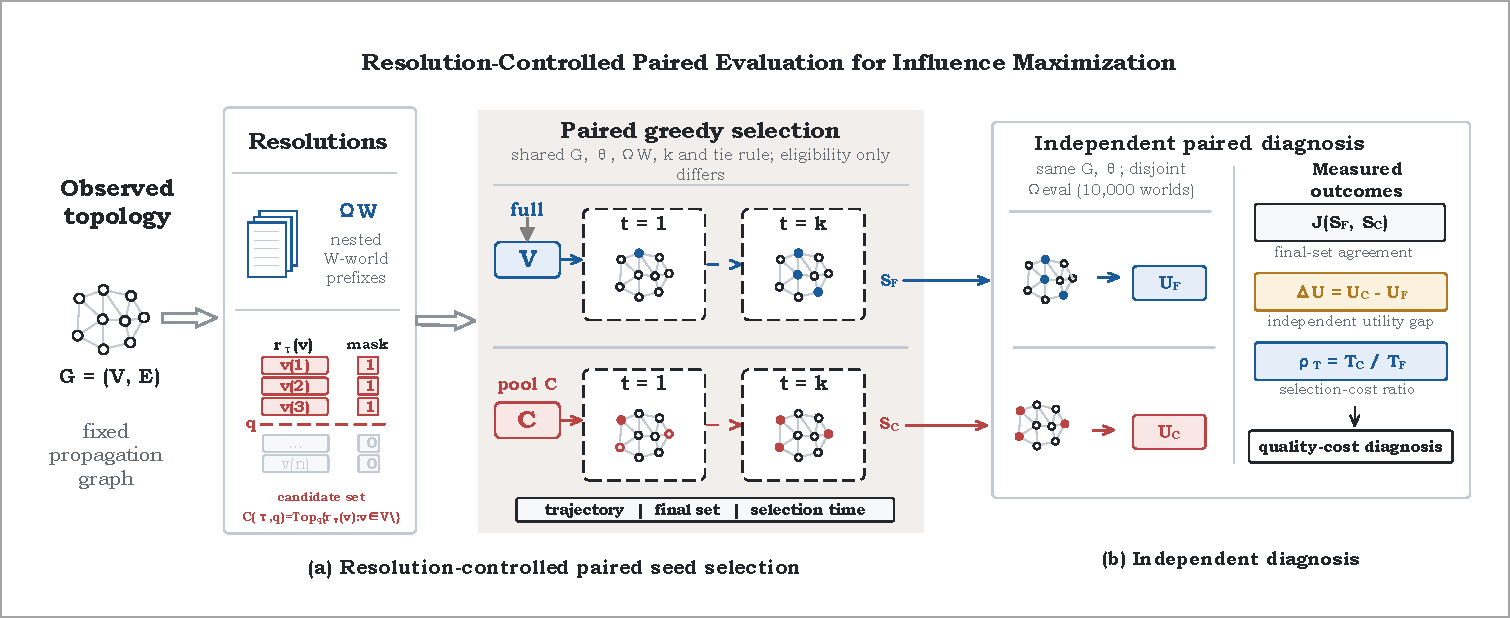
\includegraphics[width=\linewidth]{FigEvaluationMechanism.pdf}
\caption{配对评价区分选择采样、候选排名与独立效用评估。（a）两实验臂均使用相同的 $W$ 个世界选择种子，排名容差 $\tau$ 与截断值 $q$ 定义受限候选池 $C(\tau,q)$。两实验臂共享图、世界前缀、种子预算与同分规则。（b）单独且共享的 $M=10,000$ 个评估世界给出效用差 $\Delta U$，方向为受限方法减去全候选参照。集合一致性 $J$ 与选择成本比 $\rho_T$ 共同构成质量与成本比较。}\label{fig:evaluation-mechanism}
\end{figure}

\section{相关工作}
\paragraph{目标函数、采样与计算效率。}Kempe 等证明了独立级联模型下期望传播量的单调性和次模性，为贪心近似提供依据 \cite{ref1}。CELF 利用次模性避免不必要的边际收益重复评估 \cite{ref7}。StaticGreedy 在整个选择过程中复用固定的采样实现，保持一致的采样覆盖目标 \cite{ref8}。IMM 则给出具有近似保证的采样式求解器 \cite{ref2}。这些方法处理指定目标下的优化计算困难，说明需要谨慎对待采样目标，但并未直接给出某个截断排名排除节点后所造成的效用后果。本文固定模拟器与贪心规则，改变候选资格、共享选择预算或排名容差。

\paragraph{影响力估计与种子选择策略。}Rui 等利用多层邻域信息估计影响力 \cite{ref12}，Fan 等采用离散哈里斯鹰优化进行种子选择 \cite{ref13}。Ko 等的 MONSTOR+ 预测未见图上的传播量 \cite{ref19}。这些研究提供了不同的影响力估计或种子集合搜索方式，其算法目标与仅将固定排名作为种子资格过滤器进行评价不同。在后一种设置中，贪心选择仍在完整传播图上评估传播，候选覆盖率也成为比较的一部分。因此，本文区分排名在定义候选池中的作用，以及模拟器在评估所选种子中的作用。

\paragraph{评价设置与仍需回答的问题。}Li 等综述了影响力最大化方法 \cite{ref9}，Arora 等在基准研究中比较了这些方法的质量与计算成本 \cite{ref16}。Yanchenko 等综述了时间网络上的问题形式 \cite{ref11}；Aral 和 Dhillon 研究了实证影响力模型 \cite{ref15}。这些研究方向共同表明，算法比较需要放在相应传播模型、网络表示和评价设置中理解。本文在观测拓扑上模拟传播，考察该计算设置内部的敏感性，并不估计现实中实际发生的社会影响。

对于截断排名，候选池的构建与种子的选择分属两个计算环节。排名决定哪些节点进入搜索，采样目标决定从中选出哪些种子。本文分别改变这两个环节的设置，在独立评估世界上测量传播差异。

\section{研究方法}
我们在同一传播图上比较全候选与受限候选贪心选择。本节定义选择目标、评估指标和计时范围。网络特征及参数见第~\ref{sec:experimental-setup}节。
\subsection{控制分辨率的配对选择}
设 $G=(V,E)$ 为有向传播图，$S$ 为大小为 $k$ 的种子集合。在独立级联模型中，每个新激活节点都有一次机会，以概率 $p$ 激活其每个尚未激活的出向邻居。传播在 $h$ 轮后停止。对随机世界 $\omega$，用 $f_h(S;\omega)$ 表示包括种子在内的激活节点总数。贪心选择采用以下采样目标：
\begin{equation}
\widehat\sigma_W(S)=\frac{1}{W}\sum_{w=1}^{W}f_h(S;\omega_w).
\end{equation}
每轮贪心选择枚举所有尚未选中的合资格节点，并选择整数总分 $W\widehat\sigma_W$ 最大的节点。同分时按原始节点 ID 的字典序处理。全候选选择采用 $C=V$，受限选择采用 $C\subseteq V$；所有节点均保留在传播图中。一条随机路径标识一次计算重复及其随机世界族；一个实验条件固定图、路径和实验设置；一个实验臂规定该条件下的种子候选资格规则。全候选臂和受限臂共享 $G$、世界前缀、$k$ 与同分规则。

在预算扫描中，$W$ 同时控制全候选参照和所有受限实验臂的种子选择。每个实验臂在各个 $W$ 下重新选择种子，并使用相同的嵌套世界前缀。在给定排名设置下，候选池在不同 $W$ 间保持固定；排名容差 $\tau$ 和池大小 $q$ 单独控制。因此，相对差异反映两类选择过程的共同变化，不能仅归因于参照的改善。

Degree 按不同出向邻居的数量排名。PageRank 使用无权有向拓扑及 NetworkX 3.5 的默认设置：阻尼系数 .85、均匀的个性化分布和悬挂节点处理、容差 $10^{-6}$，最多迭代 100 次 \cite{networkxpr}。其停止条件为相邻两次向量的 $L_1$ 变化小于 $n\tau$，其中 $n=|V|$。分数按降序排列，同分时采用字典序。前 $q$ 名候选池包含 $q=\min(n,4k)$ 或 $q=\lceil .05n\rceil$ 个节点。在存在事件计数的网络中，历史加权度统计观测到的出向事件数。每个图与路径组合独立生成三个随机候选池，并在不同预算与耦合对照之间保持不变。

\subsection{世界耦合与独立评估}\label{sec:coupling}
主要选择世界共享以世界、传播步、源节点和目标节点为索引的随机抽样。对每个固定种子集合，这种耦合保留独立级联模型的边际分布，但实现后的有限世界目标可能不具单调性。例如，将某个中间节点设为初始激活节点，可能使其出向激活尝试提前到具有不同采样结果的传播步。在线补充材料 1 给出了明确反例。另设的固定边对照对每条边在每个世界中只抽样一次，其有限目标是各世界中沿至多 $h$ 条边可达的节点覆盖量，具有单调性和次模性。两种实现均使用完整枚举。

随着 $W$ 增大，选择世界标识符形成嵌套前缀。外部研究及 520 条件历史扩展对每个图、路径与耦合组合使用 $M=10,000$ 个评估世界；它们与选择世界不重叠，并在不同实验臂与预算下保持不变。随机键也将不同图、路径以及候选池随机化彼此区分。每种耦合方式下的方法均与该耦合方式自身的全候选参照比较。

对受限种子 $S_C$ 和全候选参照种子 $S_F$，定义世界 $i$ 上的配对评估差为 $d_i=f_h(S_C;\eta_i)-f_h(S_F;\eta_i)$。两个集合均在相同的 $W$ 下选出；$d_i$ 为正表示受限方法的传播量更高。图~\ref{fig:evaluation-mechanism} 中的效用差为
\begin{equation}
\widehat\Delta=\frac{1}{M}\sum_{i=1}^{M}d_i,
\qquad \operatorname{SE}_{\rm MC}=s(d_i)/\sqrt M.
\end{equation}
区间 $\widehat\Delta\pm1.96\operatorname{SE}_{\rm MC}$ 描述给定已选集合时的条件蒙特卡洛不确定性。路径间标准差描述不同计算路径之间的变异，其中也包含有限评估带来的噪声。在进行上述任一种计算之前，先在每条路径内对三个随机池的评估向量取平均。

我们报告有序轨迹一致性、最终集合一致性、Jaccard 相似度和首次分歧轮次。增量传播量为总传播量减去 $k$；增量传播损失百分比为 $-100\widehat\Delta/(\widehat\sigma_{\rm full}-k)$。负损失表示受限集合的评估结果更高。所有观测分母均为正。

冻结的主要检验在 $W=1280$ 时，将 Degree-4k、PageRank-4k 和路径内随机池均值分别与全候选选择比较。每项比较采用双侧精确符号检验；Holm 校正在每个图内覆盖这三项比较。零差值不纳入检验，并单独报告。覆盖率、耦合和预算转移分析均为描述性分析；世界与路径都不是独立的网络样本。

\subsection{实现与成本测量}
Numba 实现保存候选节点 ID、已选序列、各轮整数总分和逐世界评估值。复现与核验流程见在线补充材料 1。\footnote{OpenAI Codex 协助完成了基础代码与文稿起草。}

选择时间包括贪心搜索和候选节点的字典序排序，但不包括图准备、世界生成和评估。我们还估计包含独立评估的暖进程运行成本：将单独测量的解析、建图以及一个方法的排名和候选池生成成本，与记录的选择世界准备、种子选择、评估世界准备及评估成本相加。准备阶段采用五次重复的中位数。上述分项拼接估计不包括导入、即时编译、下载和输出写入。

在路径 1101、$W=320$ 下进行五次随机顺序的重复计时，以评估时间变异。成本比较采用本实现逐轮完整枚举的全候选参照。较紧 PageRank 容差的结果仅用于质量敏感性分析；计时比较采用默认容差。

\section{实验设置}\label{sec:experimental-setup}
\paragraph{输入与输出。}每次运行输入处理后的图$G$及边方向、$k$、$p$、$h$、共享选择预算$W$和候选规则。排名容差$\tau$与截断值$q$决定受限候选池$C$，传播图保持完整。选择阶段输出$k$个种子的有序序列、最终集合及选择耗时。独立评估以该集合和$M$个留出世界为输入，输出总传播量、增量传播量及相对同预算全候选参照的配对差值。表~\ref{tab:primary}和表~\ref{tab:case}将这些输出与候选数量及原始节点编号对应起来。

\subsection{网络与预处理}
我们在查看种子集合或效用之前，选定三个较大的 SNAP 拓扑 \cite{snap}：CollegeMsg 通信网络、ca-GrQc 合作网络和 wiki-Vote 投票网络。表~\ref{tab:data} 给出处理后的规模与候选覆盖率。所有保留的连通分量均纳入实验。
\begin{table}[htbp]
\caption{处理后的外部网络与候选覆盖率。弧指有向传播弧；5\% 候选池包含 $\lceil .05n\rceil$ 个节点。}\label{tab:data}
\begin{tabular}{lrrrr}
\toprule
网络 & 节点数 & 弧数 & 4k 占比 & 5\% 池大小 \\
\midrule
CollegeMsg & 1,438 & 13,397 & 1.391\% & 72 \\
ca-GrQc & 5,241 & 28,968 & 0.382\% & 263 \\
wiki-Vote & 7,115 & 103,689 & 0.281\% & 356 \\
\bottomrule
\end{tabular}
\end{table}

CollegeMsg 记录带时间戳的发送者至接收者消息 \cite{college}。我们对 58,911 个不同时间戳排序，保留前 $\lfloor .65\times58,911\rfloor=38,292$ 个完整时间戳组，纳入截至 Unix 时间戳 1085640224 的事件。去除发给自身的消息后，剩余 38,939 个事件。重复的发送者--接收者对计入历史出向消息数，但在传播图中仅形成一条弧。传播采用统一概率 $p$，不依赖消息次数。

ca-GrQc 的边连接共同作者 \cite{grqc}；我们去除自环、对节点对去重，并建立双向弧。在移除自环后收集节点，因此排除了仅出现在自环中的节点 12295，得到 5,241 个节点，而非数据源页面的 5,242 个。wiki-Vote 的弧从投票者指向被投票者 \cite{signed,links}；去除自环与重复弧，不反转其余弧的方向。沿这些弧进行出向传播是模拟假设。两个静态数据集提供拓扑信息；历史加权排名仅用于具有事件计数的数据集。我们保留所有弱连通分量：CollegeMsg 为 2 个，ca-GrQc 为 354 个，wiki-Vote 为 24 个。原始 ID 以字符串保存，图索引、排名同分和贪心同分均按字典序处理。数据清单提供原始文件和预处理图的哈希。

历史背景来自四个含 75--402 个节点的接触图，分别由工作场所、会议和肯尼亚乡村接触数据构建 \cite{ref3,ref4,ref5,ref6}。我们区分四层证据：最初的 42 条件研究、520 条件历史扩展、下述外部实验矩阵，以及事后 PageRank 精度控制。历史扩展在每张接触图上使用十条路径，增加了最高至 $W=5120$ 的预算扫描、四种对 $(p,h)$ 的局部调整、固定边采样、更大的种子预算，以及两个固定的 2,000 节点合成实例 \cite{ref17,ref18}。参数对照复用预算扫描中的默认条件。在线补充材料 1 单独报告完整实验覆盖与描述性结果。

\subsection{主要实验矩阵与数值敏感性控制}
表~\ref{tab:settings} 给出外部研究设计。实验条件改变图、路径、选择预算与耦合方式，其余传播设置固定。三个图、五条路径和三个选择预算构成 45 个主要条件，另有九个固定边条件作为匹配的耦合对照。每个条件均包括全候选选择、Degree-4k、PageRank-4k、Degree-5\%、PageRank-5\% 以及三个 random-4k 池；CollegeMsg 还包括按出向消息次数构建的 Weighted-4k 和 Weighted-5\% 池。因此，每个图有 18 个条件，CollegeMsg 每条件有 10 个实验臂，两个静态图各有 8 个，共 $18(10+8+8)=468$ 个实验臂。全部 54 个条件均已完成并保留。

\begin{table}[htbp]
\caption{外部实验设置。路径标识各图上的计算重复。}\label{tab:settings}
\begin{tabularx}{\linewidth}{lX}
\toprule
项目 & 设置 \\
\midrule
传播 & 独立级联；统一 $p=0.01$；传播期限 $h=3$；$k=5$ 个种子 \\
主要选择 & 按步耦合；$W\in\{80,320,1280\}$；路径 1101--1105 \\
独立评估 & 每个图/路径/耦合组合使用 $M=10,000$ 个世界；实验臂与预算之间共享 \\
候选池大小 & $4k=20$；另一设置为 $\lceil0.05n\rceil$；每条路径有三个大小为 20 的随机池 \\
耦合对照 & 固定边；$W=320$；路径 1101--1103 \\
默认 PageRank & 阻尼系数 0.85；$\tau=10^{-6}$；最多迭代 100 次 \\
精度控制 & $\tau=10^{-12}$；最多迭代 1,000 次；在 $10^{-14}$ 下检查池成员稳定性 \\
重复计时 & 每个实验臂重复五次；路径 1101，$W=320$；实验臂顺序随机化 \\
\bottomrule
\end{tabularx}
\end{table}

外部网络的选择预算从80增至1280个世界。每个预算下，两种方法均选择五个种子，传播概率$p=.01$，期限$h=3$。历史接触图的预算扫描延伸至$W=5120$。

事后PageRank精度对照复用原五条路径。在每个$W$下，以$10^{-12}$容差和最多1,000次迭代重新选取受限种子，再在同一组评估世界上与该预算的原全候选参照比较。容差取$10^{-12}$和$10^{-14}$时，候选池成员完全相同。两阶段精度对照的设计见在线补充材料1。

\subsection{随机化、执行与可复现性}
世界标识符区分不同图、路径以及选择/评估世界族。增大 $W$ 只追加选择世界，不重新采样已有前缀；同时检查选择与评估标识符是否重叠。随机候选池采用单独的随机化键，并在不同预算和耦合对照间保持固定。在线补充材料 1 的“可执行复现流程”给出了精确哈希键、标识符构造和哈希值到随机抽样的映射。

实验在 Windows 上使用单个串行工作进程，环境包括 Python 3.13.0、NumPy 2.3.3、NetworkX 3.5、SciPy 1.16.1 和 Numba 0.68.0。BLAS/OpenMP 线程数均限制为一。计时条件执行前完成 JIT 预热；随机化实验臂顺序以减少系统性顺序效应。记录的主机具有 20 个物理 CPU 核心和约 32 GiB 内存。

\section{研究结果}
\subsection{表面上的预算反转依赖排名精度}
在ca-GrQc上，PageRank-4k与全候选参照的比较方向是否取决于排名容差？默认容差下，$W=80$时，按路径计算的相对增量传播量平均高于同预算参照5.61\%，在$W=320$和1280时分别低于参照2.53\%和5.07\%。收紧容差后，三个预算下的均值分别高于参照11.25\%、2.96\%和0.54\%（图~\ref{fig:precision-budget}）。

收紧容差后，节点1488和19865退出20节点候选池，17655和6610进入。在每个预算下，这一替换都改变了全部五条路径的最终种子集合（表~\ref{tab:precision-output}）。在$W=1280$时，严格容差受限方法减全候选参照的传播差值平均为$+0.02608$个节点，各路径从$-0.0408$到$+0.1789$（标准差0.09155）。固定严格容差候选池后，$W$从80增至320时有3/5条路径的种子集合改变，从320增至1280时有2/5条改变。

CollegeMsg 在每个预算下的默认容差与较紧容差候选池、种子和评估结果均相同，损失仍为 9.33\%、8.52\% 和 9.01\%。wiki-Vote 有一个候选节点发生变化，但较紧容差下的损失仍为 74.05\%、74.05\% 和 73.96\%。

\begin{table}[htbp]
\caption{ca-GrQc PageRank-4k的精度控制。每个预算使用原五条路径；差值为受限方法减同预算全候选参照，单位为节点。SD为路径间标准差；集合变化指固定预算下默认与严格容差之间的变化。}\label{tab:precision-output}
\centering\begin{tabular}{rrrr}\toprule
$W$ & 默认差值（SD） & 严格差值（SD） & 集合变化 \\ \midrule
80 & +0.23606 (0.27402) & +0.48570 (0.24999) & 5/5 \\
320 & -0.12632 (0.18077) & +0.13804 (0.17387) & 5/5 \\
1280 & -0.25082 (0.07636) & +0.02608 (0.09155) & 5/5 \\
\bottomrule\end{tabular}
\end{table}

\begin{figure}[t]
\centering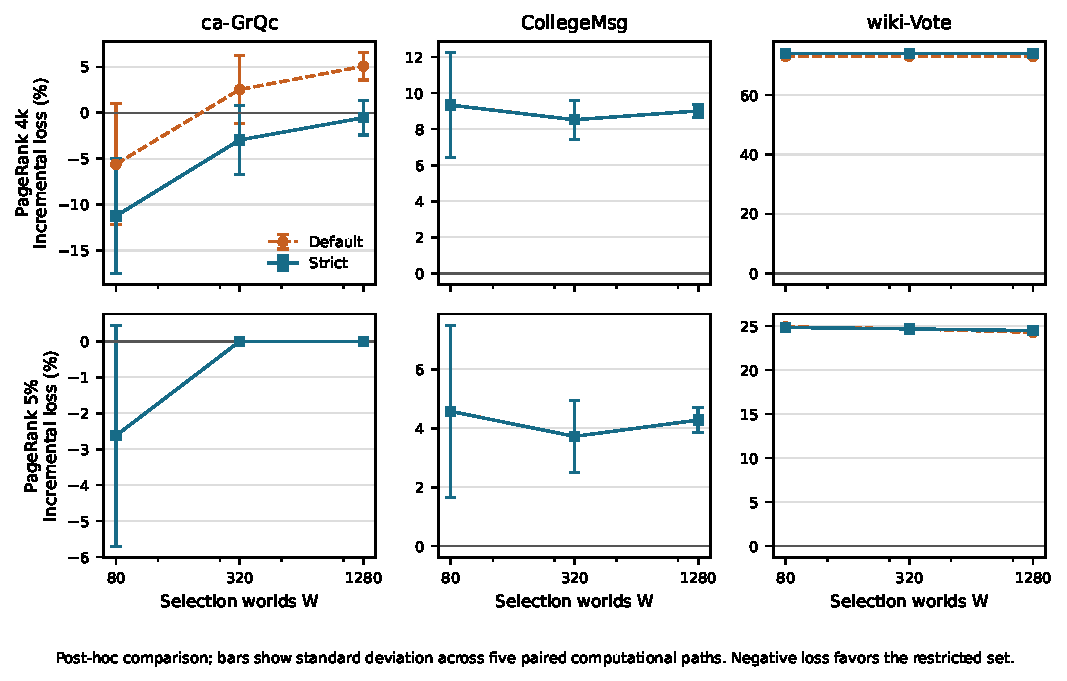
\includegraphics[width=\linewidth]{Fig4.pdf}
\caption{选择预算与排名精度对候选限制质量产生不同影响。每个 $W$ 下，受限方法均与该预算下选出的全候选参照比较；独立评估世界保持固定。点为五条配对路径的平均增量传播损失，误差线为路径标准差。图中的 Default 和 Strict 分别表示容差 $10^{-6}$ 和 $10^{-12}$；候选成员在 $10^{-12}$ 与 $10^{-14}$ 间保持不变。负损失表示受限集合的评估结果更高。收紧 PageRank 容差后，ca-GrQc 的默认反转消失，而有向网络上的损失仍存在。这是事后配对敏感性分析。}\label{fig:precision-budget}
\end{figure}

\subsection{参照集合变化不能决定传播量变化}
对于全候选参照，我们逐路径比较$W=1280$与$W=320$时所选种子的传播量，差值取高预算减低预算（图~\ref{fig:transitions}）。ca-GrQc的五个集合全部改变，平均差值为$+0.12720$个节点，逐路径差值在$-0.0266$至$+0.2411$之间。CollegeMsg有一个集合改变，全部五条路径平均增加0.05336个节点。在wiki-Vote上，部分选择顺序改变，但各路径的最终集合相同，配对传播差值均为零。

六个发生变化的集合中，四个的逐点 95\% 条件蒙特卡洛区间完全位于零以上；ca-GrQc 的另两个区间包含零。九个未变化集合的评估向量完全相同。

在历史按步耦合比较中，预算从 $W=1280$ 增至 5120 时，16/40 个集合发生变化，高预算减低预算的平均传播量变化为 0.01111 个节点，范围为 $-0.0383$ 至 $+0.1180$。历史固定边参照也发生变化：从 $W=320$ 增至 1280 时，29/40 个集合变化，高预算减低预算的平均传播量变化为 0.061845 个节点，范围为 $-0.0110$ 至 $+0.2572$。每项预算转移均在自身耦合方式内使用共享的评估世界族。由于两项比较的预算区间不同，不能用其平均变化估计耦合效应。
\begin{figure}[t]
\centering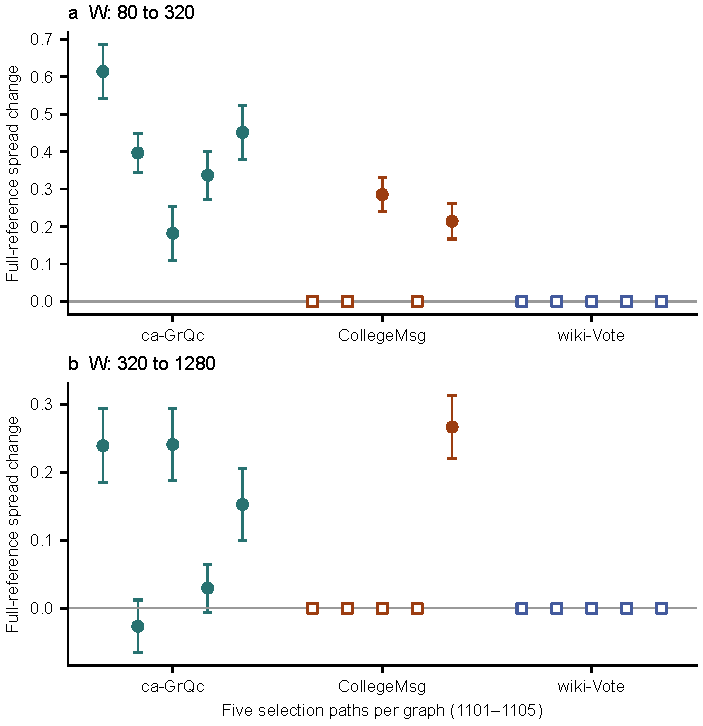
\includegraphics[width=\linewidth]{Fig2.pdf}
\caption{参照集合变化与独立传播量变化，差值为高预算减低预算的全候选参照传播量。实心圆表示最终集合变化，空心方块表示集合未变。每个图内，路径 1101--1105 从左至右排列。误差线为根据 10,000 个配对世界计算的未经校正的 95\% 条件蒙特卡洛区间。各面板采用不同纵轴尺度，以显示较小的变化；区间以已选集合为条件，不描述网络间变异。}\label{fig:transitions}
\end{figure}

\subsection{排名一致性受覆盖率与网络背景限定}
在 $W=1280$ 时，Degree-4k 仅用 20 个候选节点便复现了三个外部图上的全部全候选参照轨迹（表~\ref{tab:primary}）。默认 PageRank-4k 未匹配任何轨迹，在 ca-GrQc、CollegeMsg 和 wiki-Vote 上的平均增量传播损失分别为 \GrqcPRLoss{}\%、\CollegePRLoss{}\% 和 \WikiPRLoss{}\%。历史扩展中的 PageRank 一致性明显更广：在 $W=5120$ 时匹配 40/40 条轨迹，而基于度的方法为 39/40。外部结果因此限定了接触图排名结果的迁移范围。
\begin{table}[htbp]
\caption{各外部网络在 $W=1280$ 下的实际输出（五条路径均值）。PR 使用默认容差。增量传播量扣除 $k=5$ 个种子；差值为受限方法减全候选参照，单位均为节点。一致性为相同选择顺序的路径数。}\label{tab:primary}
\centering\begin{tabular}{lrrrr}\toprule
网络 / 方法 & 候选数 & 增量传播量 & 差值 & 一致性 \\ \midrule
\multicolumn{5}{l}{\textit{ca-GrQc}} \\
Full & 5241 & 4.934 & --- & --- \\
Degree-4k & 20 & 4.934 & +0.00000 & 5/5 \\
PR-4k & 20 & 4.683 & -0.25082 & 0/5 \\
PR-5\% & 263 & 4.934 & +0.00000 & 5/5 \\
\addlinespace
\multicolumn{5}{l}{\textit{CollegeMsg}} \\
Full & 1438 & 10.072 & --- & --- \\
Degree-4k & 20 & 10.072 & +0.00000 & 5/5 \\
PR-4k & 20 & 9.164 & -0.90780 & 0/5 \\
PR-5\% & 72 & 9.641 & -0.43094 & 0/5 \\
\addlinespace
\multicolumn{5}{l}{\textit{wiki-Vote}} \\
Full & 7115 & 55.736 & --- & --- \\
Degree-4k & 20 & 55.736 & +0.00000 & 5/5 \\
PR-4k & 20 & 15.043 & -40.69334 & 0/5 \\
PR-5\% & 356 & 42.206 & -13.53012 & 0/5 \\
\addlinespace
\bottomrule\end{tabular}
\end{table}

在wiki-Vote的路径1101上，Degree从20个候选节点中选出的五个种子及其顺序，与在全图7,115个节点中搜索的结果一致（表~\ref{tab:case}），平均总传播量均为60.8455个节点。候选数同为20时，默认PageRank选出的五个种子均与参照不同，平均传播量为19.9366个节点。候选池扩大到356个节点后，传播量增至47.2095。各网络的五路径比较见表~\ref{tab:primary}。
\begin{table}[htbp]
\caption{wiki-Vote 的输入与输出案例：路径1101，$k=5$、$p=.01$、$h=3$、$W=1280$、$M=10,000$，按步耦合。输入图含7,115个节点和103,689条弧。PR采用默认容差；箭头表示选择顺序。传播量是独立模拟均值，包含种子。}\label{tab:case}
\begin{tabularx}{\linewidth}{lXr}\toprule
方法 & 输出的种子顺序 & 总传播量 \\ \midrule
Full & $2565\to 766\to 11\to 457\to 2688$ & 60.8455 \\
Degree-4k & $2565\to 766\to 11\to 457\to 2688$ & 60.8455 \\
PR-4k & $3352\to 2237\to 2328\to 2654\to 1297$ & 19.9366 \\
PR-5\% & $2565\to 1166\to 1549\to 1374\to 5524$ & 47.2095 \\
\bottomrule\end{tabularx}
\end{table}

在最高测试外部预算下的主要比较中，默认 PageRank-4k 和路径内 random-4k 均值相对全候选选择的每个差值都为负，未经校正的符号检验 $p=.0625$，图内 Holm 校正后 $p=.1875$。Degree-4k 与全候选选择的差值严格为零。五条路径使双侧符号检验可达到的最小值限制在 .0625。在线补充材料 1 报告配对效应量、敏感性控制和完整检验结果。

将默认 PageRank 池增至 5\% 后，在 $W=1280$ 时复现了 ca-GrQc 的全部五个参照，并将 CollegeMsg 的损失从 \CollegePRLoss{}\% 降至 \CollegePRfiveLoss{}\%。wiki-Vote 的损失从 \WikiPRLoss{}\% 降至 \WikiPRfiveLoss{}\%，仍高于全候选参照增量传播量的五分之一。同预算下，CollegeMsg 的历史加权池由 4k 下平均差 $-0.25224$ 个节点，变为 5\% 下完全复现参照。在这些比较中，增加覆盖率有所帮助，但作用随网络而异。

在 wiki-Vote 上，默认 PageRank 前 20 个节点的平均入度为 249.75、出度为 56.2；按度排名的前 20 个节点平均入度为 70.3、出度为 489.25。在任一 $W=1280$ 路径上，PageRank-4k 候选池都不包含五个全候选参照种子中的任何一个，而其 5\% 候选池仅包含一个。在线补充材料 1 给出了种子层面的图示和完整覆盖率比较。

\subsection{指定计时范围下保持参照结果的计算节省}
在 $W=1280$ 时，相对本实现的全候选参照，Degree-4k 将实测选择时间降低 98.40--99.67\%，同时复现全部参照轨迹（表~\ref{tab:cost}）。计入准备阶段、两类世界准备及独立评估后，分项拼接的成本节省为 \CollegeDegreeSaving{}--\WikiDegreeSaving{}\%。
\begin{table}[htbp]
\caption{Degree-4k 在 $W=1280$ 下的成本，取五条路径平均。Full 与 Degree 列为实测选择时间。最后一列估计包含准备阶段、选择及评估世界准备、种子选择和独立评估的成本节省。这些暖进程拼接成本排除导入、JIT 编译、下载和输出写入，并非直接端到端计时。}\label{tab:cost}
\begin{tabular}{lrrrr}
\toprule
网络 & Full（s） & Degree（s） & \shortstack{选择阶段\\节省（\%）} & \shortstack{含评估成本\\节省（\%）} \\
\midrule
ca-GrQc & 23.53 & 0.109 & 99.54 & 92.77 \\
CollegeMsg & 5.89 & 0.094 & 98.40 & 86.59 \\
wiki-Vote & 158.94 & 0.520 & 99.67 & 96.26 \\
\bottomrule
\end{tabular}
\end{table}


在 $W=1280$ 时，Degree-4k 在每条路径上均满足相对全候选选择的零点估计损失阈值。默认 PageRank-4k 在 ca-GrQc 和 CollegeMsg 上满足 10\% 阈值，但在 wiki-Vote 的每条路径上均未满足 20\% 阈值。所有随机池的路径均值都未满足 20\% 阈值。在线补充材料 1 报告全部六个冻结阈值（0、1、2.5、5、10 和 20\%）及相应成本估计；它们是描述性标准，而非经实际应用验证的可容忍损失。

\subsection{参数与耦合对照限定结论范围}

在 $W=320$ 的外部固定边对照中，默认 PageRank-4k 减去固定边全候选参照的平均传播差值，在 ca-GrQc、CollegeMsg 和 wiki-Vote 上分别为 $-0.16240$、$-0.93417$ 和 $-40.57597$ 个节点。Degree-4k 分别复现 1/3、3/3 和 3/3 条对应轨迹。PageRank 损失在此对照下仍存在，而部分参照一致性结果发生变化。在线补充材料 1 提供完整对照路径和重复计时。

在 $W=320$ 的 160 个历史非默认参数条件中，Degree-4k 和 PageRank-4k 分别复现 117 和 132 条全候选参照轨迹。Weighted-4k 减去全候选选择的配对传播差值中，117 个为负，43 个为正。

在 $W=1280$ 的历史固定边采样下，Degree-4k 和 PageRank-4k 分别匹配固定边全候选参照的 38/40 和 40/40 条轨迹，Weighted-4k 匹配 5/40。
\FloatBarrier

\section{讨论}
\subsection{ca-GrQc传播差值反转的条件}
在默认PageRank容差下，仅看ca-GrQc的预算扫描，会得出受限方法在最低预算优于全候选参照、在最高预算落后于参照的判断。替换两个候选节点就改变了这一判断。固定$W$时，两种容差对应的全候选参照、采样目标和评估世界相同，因此平均传播差值的反转依赖哪些节点有资格成为种子。即使固定较严格的候选池，增加$W$仍会改变种子，最高预算下各路径的传播差值也有正有负。

StaticGreedy在搜索过程中复用固定的采样实现\cite{ref8}。本文的两种方法也共享选择样本，但排名和截断发生在搜索之前。报告截断处发生替换的候选节点，才能追踪这一环节造成的差异。

\subsection{选择顺序、最终集合与传播量}
选择顺序记录贪心搜索每一轮的决策，传播模型的输入则是最终种子集合。在wiki-Vote上，只要两个预算返回同一集合，即使选择顺序改变，每个评估世界的传播计数也相同。成员改变后，差值的方向要由独立评估确定：在ca-GrQc上，高预算选出的种子在部分路径触达更多节点，在另一些路径触达更少节点。

\subsection{候选覆盖率与排除节点的代价}
在wiki-Vote上，默认PageRank排名前20的候选池排除了全部五个参照种子。扩大到前356个节点后，一个参照种子进入候选池。扩大后的候选池至多能选中一个参照种子，但五条路径的平均总传播量已从20.04268增至47.20590个节点，全候选参照为60.73602个节点。

两个20节点候选池选中了有向图上的不同节点。PageRank候选节点收到的投票较多，度候选节点则有较多不同的出向邻居。模拟传播沿投票者到被投票者的方向进行，观察到的损失与这种方向差异一致。在同一拓扑上反转传播方向，可以直接检验这一解释。

Arora等将影响力最大化方法的传播量与运行时间结合比较\cite{ref16}。本文的计时结果对应具体的选择输出：Degree-4k省去了大部分候选节点评分，在最高预算的全部15条路径上仍复现参照序列。wiki-Vote上的默认PageRank-4k同样只搜索20个候选节点，平均增量传播损失却达到73.01\%。表~\ref{tab:cost}分别列出选择阶段实测时间和计入准备与评估的成本估计。

\subsection{比较范围}
外部比较覆盖三张观测拓扑，模拟设置为$k=5$、$p=.01$、$h=3$、$W\le1280$。历史接触图还考察了其他传播概率、期限和种子数，但候选覆盖率也更高：$k=20$时，Kenya的候选池包含全部节点，invs2013保留80/91个节点。这些条件下的参照一致性，与wiki-Vote上仅保留20个候选节点时的一致性，所对应的搜索范围差别很大。

事后容差比较使用按步耦合下原有的五条路径。若在固定边采样下对两种容差进行配对比较，可以检验ca-GrQc的结果在该采样方式下是否仍然成立。

\section{结论}
在ca-GrQc上，PageRank截断处两个候选节点的替换，使不同选择预算之间的平均差值反转消失。在wiki-Vote上，扩大候选池后虽然只纳入一个参照种子，却恢复了部分传播量。评价候选限制时，同时报告排名选入哪些候选节点、最终种子触达多少节点，可以区分这两种现象。在所考察的三张外部图上，Degree-4k以更低的实测选择成本复现了最高预算的参照序列。

\paragraph{补充信息。}在线补充材料 1 包含外部结果矩阵、精度与方向诊断、损失--成本曲线，以及单独列出的历史覆盖率、参数、耦合与次要对照表，并提供复现细节。
\section*{声明}
\paragraph{基金支持。}本研究获得省级大学生创新创业训练项目支持。
\paragraph{利益冲突。}作者声明不存在利益冲突。
\paragraph{作者贡献。}Jiayue Sun：概念构思、方法设计、软件、验证、正式分析、研究实施、数据整理、可视化及初稿写作。Binbin Yong：指导、方法设计、项目管理及审阅与修改。Junjie An：软件、数据整理及审阅与修改。Tianyu Bo：验证、可视化及审阅与修改。Shuai Li：正式分析、验证及审阅与修改。全体作者已阅读并批准最终稿件，同意向 \textit{Computing} 投稿。
\paragraph{数据可用性。}第三方数据集可按照其访问条款从所引数据提供方获取，本文不再分发这些数据。投稿材料附有来源记录、预期 SHA-256 哈希和预处理说明。
\paragraph{代码可用性。}冻结源码快照、配置、验证程序、分析脚本、逐条件输出和图表源数据随投稿材料提供，供编辑及同行评审查阅。
\begin{thebibliography}{99}
\bibitem{ref1} Kempe D, Kleinberg J, Tardos É (2003) Maximizing the spread of influence through a social network. In: ACM SIGKDD, pp 137--146. \url{https://doi.org/10.1145/956750.956769}

\bibitem{ref7} Leskovec J, Krause A, Guestrin C, Faloutsos C, VanBriesen J, Glance N (2007) Cost-effective outbreak detection in networks. In: KDD, pp 420--429. \url{https://doi.org/10.1145/1281192.1281239}

\bibitem{ref8} Cheng S, Shen H, Huang J, Zhang G, Cheng X (2013) StaticGreedy: solving the scalability-accuracy dilemma in influence maximization. In: CIKM, pp 509--518. \url{https://doi.org/10.1145/2505515.2505541}

\bibitem{ref2} Tang Y, Shi Y, Xiao X (2015) Influence maximization in near-linear time: a martingale approach. In: ACM SIGMOD, pp 1539--1554. \url{https://doi.org/10.1145/2723372.2723734}

\bibitem{ref12} Rui X, Yang X, Fan J, Wang Z (2020) A neighbour scale fixed approach for influence maximization in social networks. Computing 102:427--449. \url{https://doi.org/10.1007/s00607-019-00778-5}

\bibitem{ref13} Fan C, Wang Z, Zhang J, Zhao J, Rui X (2024) Influence maximization in social networks based on discrete harris hawks optimization algorithm. Computing 106:327--351. \url{https://doi.org/10.1007/s00607-023-01207-4}

\bibitem{ref19} Ko J, Kim S, Lee K, et al. (2025) Inductive influence estimation and maximization over unseen social networks under two diffusion models. Data Mining and Knowledge Discovery 39:55. \url{https://doi.org/10.1007/s10618-025-01137-z}

\bibitem{ref9} Li Y, Fan J, Wang Y, Tan K-L (2018) Influence maximization on social graphs: a survey. IEEE Transactions on Knowledge and Data Engineering 30:1852--1872. \url{https://doi.org/10.1109/TKDE.2018.2807843}

\bibitem{ref16} Arora A, Galhotra S, Ranu S (2017) Debunking the myths of influence maximization: an in-depth benchmarking study. In: SIGMOD, pp 651--666. \url{https://doi.org/10.1145/3035918.3035924}

\bibitem{ref11} Yanchenko E, Murata T, Holme P (2024) Influence maximization on temporal networks: a review. Applied Network Science 9:16. \url{https://doi.org/10.1007/s41109-024-00625-3}

\bibitem{ref15} Aral S, Dhillon PS (2018) Social influence maximization under empirical influence models. Nature Human Behaviour 2:375--382. \url{https://doi.org/10.1038/s41562-018-0346-z}

\bibitem{networkxpr} NetworkX developers (2025) PageRank, NetworkX 3.5 documentation. \url{https://networkx.org/documentation/networkx-3.5/reference/algorithms/generated/networkx.algorithms.link_analysis.pagerank_alg.pagerank.html}. Accessed 15 October 2026

\bibitem{snap} Leskovec J, Krevl A (2014) SNAP datasets: Stanford large network dataset collection. \url{https://snap.stanford.edu/data}. Accessed 15 October 2026

\bibitem{college} Panzarasa P, Opsahl T, Carley KM (2009) Patterns and dynamics of users' behavior and interaction: Network analysis of an online community. Journal of the American Society for Information Science and Technology 60:911--932. \url{https://doi.org/10.1002/asi.21015}

\bibitem{grqc} Leskovec J, Kleinberg J, Faloutsos C (2007) Graph evolution: densification and shrinking diameters. ACM Transactions on Knowledge Discovery from Data 1(1):2. \url{https://doi.org/10.1145/1217299.1217301}

\bibitem{signed} Leskovec J, Huttenlocher D, Kleinberg J (2010) Signed networks in social media. In: CHI, pp 1361--1370. \url{https://doi.org/10.1145/1753326.1753532}

\bibitem{links} Leskovec J, Huttenlocher D, Kleinberg J (2010) Predicting positive and negative links in online social networks. In: WWW, pp 641--650. \url{https://doi.org/10.1145/1772690.1772756}

\bibitem{ref3} Génois M, Vestergaard CL, Fournet J, Panisson A, Bonmarin I, Barrat A (2015) Data on face-to-face contacts in an office building suggest a low-cost vaccination strategy based on community linkers. Network Science 3:326--347. \url{https://doi.org/10.1017/nws.2015.10}

\bibitem{ref4} Génois M, Barrat A (2018) Can co-location be used as a proxy for face-to-face contacts? EPJ Data Science 7:11. \url{https://doi.org/10.1140/epjds/s13688-018-0140-1}

\bibitem{ref5} Cattuto C, Van den Broeck W, Barrat A, Colizza V, Pinton J-F, Vespignani A (2010) Dynamics of person-to-person interactions from distributed RFID sensor networks. PLoS ONE 5:e11596. \url{https://doi.org/10.1371/journal.pone.0011596}

\bibitem{ref6} Kiti MC, Tizzoni M, Kinyanjui TM, et al. (2016) Quantifying social contacts in a household setting of rural Kenya using wearable proximity sensors. EPJ Data Science 5:21. \url{https://doi.org/10.1140/epjds/s13688-016-0084-2}

\bibitem{ref17} Barabasi A-L, Albert R (1999) Emergence of scaling in random networks. Science 286:509--512. \url{https://doi.org/10.1126/science.286.5439.509}

\bibitem{ref18} Holland PW, Laskey KB, Leinhardt S (1983) Stochastic blockmodels: first steps. Social Networks 5:109--137. \url{https://doi.org/10.1016/0378-8733(83)90021-7}
\end{thebibliography}

\end{document}
